%%%%%%%%%%%%%%%%%%%%%%%%%%%%%%%%%%%%%%%%%%%%%%%%%%%%%%%%%%%%%%%%%%
%%%%%%%% ICML 2016 EXAMPLE LATEX SUBMISSION FILE %%%%%%%%%%%%%%%%%
%%%%%%%%%%%%%%%%%%%%%%%%%%%%%%%%%%%%%%%%%%%%%%%%%%%%%%%%%%%%%%%%%%

% Use the following line _only_ if you're still using LaTeX 2.09.
%\documentstyle[icml2016,epsf,natbib]{article}
% If you rely on Latex2e packages, like most moden people use this:
\documentclass{article}

% use Times
\usepackage{times}
% For figures
\usepackage{graphicx} % more modern
%\usepackage{epsfig} % less modern
\usepackage{subfigure} 

% qdeee: for mathbb
\usepackage{amsmath}
\usepackage{amssymb}

% For citations
\usepackage{natbib}

% For algorithms
\usepackage{algorithm}
\usepackage{algorithmic}

% For sub-files
\usepackage{standalone}

\usepackage{multicol}
\usepackage{multirow} % http://ctan.org/pkg/multirow
\usepackage{hhline} % http://ctan.org/pkg/hhline

% For plots
\usepackage{epstopdf}
%\usepackage{color}

% As of 2011, we use the hyperref package to produce hyperlinks in the
% resulting PDF.  If this breaks your system, please commend out the
% following usepackage line and replace \usepackage{icml2016} with
% \usepackage[nohyperref]{icml2016} above.
\usepackage{hyperref}

% \AtBeginShipout{%
%   \ifnum\value{page}>1 %
%     \typeout{* Additional boxing of page `\thepage'}%
%     \setbox\AtBeginShipoutBox=\hbox{\copy\AtBeginShipoutBox}%
%   \fi
% }

% Packages hyperref and algorithmic misbehave sometimes.  We can fix
% this with the following command.
\newcommand{\theHalgorithm}{\arabic{algorithm}}

% Employ the following version of the ``usepackage'' statement for
% submitting the draft version of the paper for review.  This will set
% the note in the first column to ``Under review.  Do not distribute.''
\usepackage{icml2017} 

% Employ this version of the ``usepackage'' statement after the paper has
% been accepted, when creating the final version.  This will set the
% note in the first column to ``Proceedings of the...''
% \usepackage[accepted]{icml2017}


% The \icmltitle you define below is probably too long as a header.
% Therefore, a short form for the running title is supplied here:
\icmltitlerunning{Using Matrix Factorization Methods for Multiclass Classification tasks}

\begin{document} 

\twocolumn[
\icmltitle{Using Matrix Factorization Methods for Multiclass Classification Tasks}
            

% It is OKAY to include author information, even for blind
% submissions: the style file will automatically remove it for you
% unless you've provided the [accepted] option to the icml2017
% package.

% list of affiliations. the first argument should be a (short)
% identifier you will use later to specify author affiliations
% Academic affiliations should list Department, University, City, Region, Country
% Industry affiliations should list Company, City, Region, Country

% you can specify symbols, otherwise they are numbered in order
% ideally, you should not use this facility. affiliations will be numbered
% in order of appearance and this is the preferred way.
\icmlsetsymbol{equal}{*}

\begin{icmlauthorlist}
\icmlauthor{Ruslan Solovev}{equal,to}
\icmlauthor{Igor Kuralenok}{equal,to,goo}
\end{icmlauthorlist}

\icmlaffiliation{to}{University of Torontoland, Torontoland, Canada}
\icmlaffiliation{goo}{Googol ShallowMind, New London, Michigan, USA}

\icmlcorrespondingauthor{Ruslan Solovev}{solovevr@gmail.com}
\icmlcorrespondingauthor{Igor Kuralenok}{ikuralenok@gmail.com}


% You may provide any keywords that you 
% find helpful for describing your paper; these are used to populate 
% the "keywords" metadata in the PDF but will not be shown in the document
\icmlkeywords{multinomial logistic regression, matrix factorization, gradient boosting}

\vskip 0.3in
]

% this must go after the closing bracket ] following \twocolumn[ ...

% This command actually creates the footnote in the first column
% listing the affiliations and the copyright notice.
% The command takes one argument, which is text to display at the start of the footnote.
% The \icmlEqualContribution command is standard text for equal contribution.
% Remove it (just {}) if you do not need this facility.

\printAffiliationsAndNotice{}  % leave blank if no need to mention equal contribution
%\printAffiliationsAndNotice{\icmlEqualContribution} % otherwise use the standard text.
%\footnotetext{hi}

\begin{abstract} 
In this paper we introduce a new approach to multiclassification based on simultaneous build of all scoring functions in multinomial logistic regression framework. The proposed algorithm provides lightweight decision function while being on par with state-of-the-art methods in terms of prediction quality. The method is based on multinomial logistic regression and gradient boosting. The MLR allows the researcher not to bother balancing of different classes in dataset, and the boosting gives her the opportunity to control trade-off between time and model quality.
\end{abstract} 

\section{Introduction}
\label{introduction}
Classification onto more than two classes is very natural setting for many tasks. Among others we should mention text classification, object recognition, protein folds etc. There are four principal approaches to this problem known from the literature: one vs. rest, multinomial logistic regression \cite{GLM}, multiclass boosting \cite{journals/jmlr/MukherjeeS13} and using complex system of binary classifiers with associated modeling matrix \cite{Allwein00reducingmulticlass}.

Each of these families have their properties and depending on the task could be more or less effective. The simplicity of one vs. rest makes it the most popular method in everyday work of ML practician. On the other hand this simplicity in training process is offset by need of balancing the result scoring functions. This balancing is done either by count of the representatives of each class or by other methods \cite{imbalancing_classes1,imbalancing_classes2}.

Multinomial logistic regression boosting methods are the opposite extreme case. They are much easier to prepare for learning---scoring functions will be comparable by the design \cite{mlr_imbalancing}, but it takes ages to learn a strong model. The problem is that all scoring functions ($K-1$, where $K$ is number of classes) are built simultaneously and are independent. One need to make $K-1$ optimizations on each step after calculating of $|X|\times |K - 1|$ gradient values (X---training set).

Multiclass boosting allows us to split boosting process into training one weak classifier at a time balancing the weights of examples. Though one still need to solve multi-classification problem on each step which is difficult task. 

Modeling matrix approach generalize the one-vs-rest allowing one to build binary classifiers complimentary to each other. This way allows to build smaller number of decision functions than $K-1$. In this approach each binary classifier provides one bit of information on potential class of the object, combining this information we can ``decode'' the right class with much smaller number of classifiers if the binary classifier quality is high enough. The problem is that effective in terms of coding strength classifiers are often not easy to build in terms of prediction quality. There are some works about the building of the modeling matrix \cite{modelmatrix2,Zhao_sparseoutput}, however there is no good way to build it universally and it should be constructed in ad-hoc manner in most of the cases.

Our goal is to combine described approaches to get the method that is as simple as one-vs-rest, able to work with lot of classes, less sensitive to class imbalance, has light decision function to be used online. To achieve these properties we do the gradient boosting for multinomial logistic regression to find a decision function in form of single ensemble. The multinomial logistic regression particularly allows us to forget about class imbalance; gradient boosting allows one to control trade-off between time and model quality; and the simplicity of the decision function allows us to convert multi-classification into a series of regression tasks.

The later sections of the paper are organized as follows: in motivation part the idea of the method is explained on basis of existing approaches, the algorithm is described in details in Sec. 3., then goes experimental part of the research and finally conclusions and directions for future research are presented.

% The fo

% Our contribution as follows:
% \begin{itemize}
% \item We propose the GradFac multiclassification algorithm that is based on gradient boosting and matrix factorization. We show that in most cases it can reduce total count of weak models without sufficient quality degradation.
% \item We describe the main disadvantage of the new algorithm and propose two fixes: matrix columns bootstrapping and \emph{ElasticNet} factorization. 
% \item We apply the GradFac algorithm to the classic gradient boosted tree classifier on benchmark datasets.
% \end{itemize}



\section{Motivation}

Many algorithms in ML are dedicated to classification or regression tasks and the idea of employing them for multiclassification looks attractive. The modeling matrix approach formulated by Allwein, Schapire and Singer \cite{Allwein00reducingmulticlass} allows one to split this complex task into binary classification subtasks. Unfortunately the elements of the modeling matrix must be from set of $\{-1,0,1\}$ and this fact makes the optimization on this matrix much more difficult \cite{modelmatrix2,Zhao_sparseoutput}. We want to get rid of this limitation to simplify the optimization task. Another important property of this approach is that we can use it in case the number of classes is significant and it is next to impossible to train scoring function for each of them. In this case we ``code'' the class by modeling matrix row and we are able to estimate this class probability, using results of the binary classifiers.

We will look for decision function in the class of the following functions:
\begin{equation}
H_c(x) = \sum_t b_{ct} h_t(x) 
\end{equation}
where $H_c(x)$ is a scoring function for class $c$ at point $x$, $b_{ct}$ is a scalar value, associated with the class $c$ at step $t$, and $h_t(x)$ is real-valued function of $x$. The probability of class $c$ is exactly like one in multinomial logistic regression:
\begin{equation}
  P(Y = c \arrowvert x, H) =
  \begin{cases}
    \frac{ e^{H_{c}(x)} }
       { 1+\sum_{j=1}^{K-1} e^{H_{j}(x)} }
    , & c \in \{1, \ldots, K-1 \} \\

    \frac{ 1 }
       { 1 + \sum_{j=1}^{K-1} e^{H_{j}(x)} }
    , & c=K
  \end{cases}\label{eq:MLR_model}
\end{equation}
where $P(Y = c \arrowvert x, H)$ is desired probability of the class $c \in \{1\ldots K\}$ for the point $x$.

This type of decision function look very similar to those using modeling matrix: $\mathbb{B} = \{b_{ct}\}$ form the matrix itself, and the $h_t$ are some regression task solutions:
\begin{equation}
h_{t+1} = \arg \min_h \|h(X) - r_t\|.
\end{equation}
Our task is to find proper series of $(b_t, r_t)$. We use modification of the multinomial logistic regression gradient boosting for this.

\subsection{Multinomial logistic regression}
The boosting of multinomial logistic regression is a well studied topic \cite{Friedman98additivelogistic}. The multinomial regression models discriminative surfaces between classes in form of $H_{c_1}(x)=H_{c_2}(x)$, this brings probability of the class into form of (\ref{eq:MLR_model}) \cite{GLM}. The boosting approach implies the ensemble form of scoring function $H_c(x) = \sum_t h_{ct}(x)$. The target function is the following:
\begin{multline*}
	L(X\arrowvert H) = \sum_{(x,y) \in X} \log P(Y = y \arrowvert x, H) = \\
	= \sum_{(x,y) \in X} \log \frac{ I\{y \ne K \}e^{H_y(x)} + I\{y=K\} }{ 1+\sum_{c=1}^{K-1} e^{H_c(x)} }
\end{multline*}
In this case $X$ is not only features matrix, but entire set of $(x, y)$ precedents. On each step we want $h_{t + 1}(X)$ to be aligned with the $\frac{\partial L(X|H)}{\partial H_c(x)}(H_t(X))$. For simplicity one can interpret $\frac{\partial L(X|H)}{\partial H_c(x)}(H_t(X))$ as a matrix $R_t$ of size $|X|\times K-1$. Then we optimize $h_{c,t+1}$:
\begin{equation}
h_{c,t+1} = \arg \min_h \|h_c(X) - r_{ct}\|_2^2
\label{eq:MLR_boosting_step}
\end{equation}
where $r_c$ is a column of the matrix representation of gradient $R$. At this step we need to build the regression $K-1$ times and this part is the most computationally intensive. We have described the independent variant of the optimization, but it can be enhanced even further by dropping the independence assumption for certain types of decision functions (such as regression trees).

\subsection{The idea of Factorized MultiClass Boosting}
The main difference between FMCB and the multinomial regression boosting is the form of decision function. We want to optimize (\ref{eq:MLR_boosting_step}) for all classes simultaneously. Since the $l_2$ target function is additive and we can rewrite the optimization in the following form:
\begin{equation}
(h_{t+1},b_{t+1}) = \arg \min_{h,b} \sum_c \|b_ch(X) - r_{ct}\|_2^2
\end{equation}
where $b_{t+1}$---column of the future modeling matrix. We split this optimization into two steps:
\begin{equation}\begin{array}{l}
(b_{t+1},r_{t+1}) = \arg \min_{b,r} \|b r^T - R_t\|_F^2 \\
h_{t+1}	= \arg \min_{h} \|h(X) - r_{t+1}\|_2^2
\end{array}\end{equation}
According to the Eckart-Young-Mirsky theorem \cite{Eckart1936} there is exact solution of the first optimization. The second one is just a regression problem. The proposed schema will do the same optimization only when $h$ is flexible enough to bring the $\|h(X) - r_{t+1}\|$ to zero. In most cases this is not true and this fact will grow the likelihood of divergence. The details of the algorithm will be described in the next section.
\label{sec:fmcb_idea}


\begin{algorithm}[tb]
\caption{FMCBoosting}
\label{alg:boost_fmcb}
\begin{algorithmic}
\STATE {\bfseries Input:} step $\alpha$, iterations count $T$.
\STATE $H^{(0)}(x):= \mathbb{O} \in \mathbb{F}^{K-1}$ \COMMENT{initial zero model}
\STATE $\overline{x}^{(0)} := \mathbb{O} \in \mathbb{R}^{N \times (K-1)}$ \COMMENT{initial cursor}
 
\FOR{$t=1$ {\bfseries to} $T$}
 	\STATE Evaluate the gradient's $R_t=\nabla L(\overline{x}^{(t-1)})$ using (\ref{eq:grad_matrix}).
	\STATE Factorize the gradient's matrix:
			$$(b_{t},r_{t}) = \arg\min_{b,r} \|b r^T - R_t\|_F^2$$
	\STATE Train weak model $h_{t}(x)$ using $\{X,r^T\}$ as a training set and MSE as a target function:
 			$$h_{t+1}(x) = \arg\min_{h} \|h(X) - r_{t}\|_2^2$$  	
	\STATE Update model: $H^{(t)}(x) = H^{(t-1)}(x) + \alpha b^t h^{(t)}(x)$.
	\STATE Update cursor: $\overline{x}^{t} = \overline{x}^{(t-1)} + \alpha b^t h^{(t)}(X)$.
\ENDFOR    
\end{algorithmic}
\end{algorithm}

\section{Factorized MultiClass Boosting}

The proposed algorithm optimizes the likelihood function:
\begin{multline*}
	L(X\arrowvert H) = \sum_{(x,y) \in X} \log \frac{ I\{y \ne K \}e^{H_y(x)} + I\{y=K\} }{ 1+\sum_{c=1}^{K-1} e^{H_c(x)} }.
\end{multline*}
The decision takes form of vector function:
\begin{equation}
H(x) = \sum_t b_{t} h_t(x) 
\end{equation}
where $b_t$ are vectors of $K-1$ components and $h_t$ are real functions of $x$. The optimization is done iteratively. $H_c(x)$ are treated as independent variables and therefore one can get gradient of target function in terms of these variables. It is possible to present this gradient vector as a matrix. Each column of it presents gradient of the appropriate class scoring function:
\begin{equation}
\label{eq:grad_matrix}
\nabla L = 
\left(
\begin{array}{ccc}
	  \frac{ \partial L }{ \partial H_{1}(x_{1}) } 
	& \cdots 
	& \frac{ \partial L }{ \partial H_{K-1}(x_{1}) } \\

	  \vdots & \ddots & \vdots\\

	  \frac{ \partial L }{ \partial H_{1}(x_{|X|}) } 
	& \cdots 
	& \frac{ \partial L }{ \partial H_{K-1}(x_{|X|}) }
\end{array}
\right)_{|X| \times (K-1)}
\end{equation}

Each step of optimization is done as close to the $R_t = \nabla L(H_t(X))$ as possible. To do so we factorize the matrix form of the gradient $R$ by rank $1$ matrix $b h(X)^T$ using Frobenius distance as the metric:
\begin{equation}
(b_{t+1},r_{t+1}) = \arg \min_{b,r} \|b r^T - R_t\|_F^2
\label{eq:factorization_step}
\end{equation}

According to the Eckart-Young-Mirsky theorem \cite{Eckart1936}, solving (\ref{eq:factorization_step}) means finding the left and the right singular vectors of $R_t$ associated with the largest singular value of $R_t$. Therefore, one may apply the following algorithm: 
\begin{enumerate}
	\item Evaluate the singular decomposition of gradient's matrix: $R = U \Sigma V^T$
	\item Take the largest singular value $\sigma_{1}$ and associated singular vectors $u$ and $v$.
	\item Return $\overline{u}={\sigma_{1}}{\Vert v \Vert}_{2}u$ and $\overline{v}=\frac{1}{\Vert v \Vert}_{2}v$ as solution.
\end{enumerate}
In our notation $br^T = \overline{u}\overline{v}^T$. From the solutions family we choose the pair where $\|b_{t+1}\|_2 = 1$.

Experiments show that starting from some iteration, singular values become too close to each other and choice of singular vectors associated with the largest singular value becomes non-trivial. It leads to factorization error growth because the single pair of the left and the right singular vectors is no longer a meaningful characteristic of the matrix. We call this negative effect "the spreading of singular values", as the matrix is spreading across several pairs of singular vectors. To overcome this difficulty we have introduced the bias on each step. In the following chapters the implementation of the bias in form of prior (and appropriate regularization) and introduction of the noise into data will be presented.

To find the ensemble term $h_{t+1}$ we minimize the distance with factorization component $r_{t+1}$:
\begin{equation}
h_{t+1}	= \arg \min_{h} \|h(X) - r_{t+1}\|
\label{eq:minimization_step}
\end{equation}
For our experiments we have used modification of the CART algorithm for oblivious trees \cite{Gulin_winningthe} at this step.

% \begin{figure}
% \vskip 0.2in
% \begin{center}
% \centerline{\includegraphics[width=\columnwidth]{figures/factorization_error_rate.jpg}}
% \caption{Factorization error rate growth with number of iterations of FMCB.}
% \end{center}
% \label{fig:factorization-effectiveness}
% \vskip -0.2in
% \end{figure}

\subsection{Bias in factorization}

\begin{figure}
\vskip 0.2in
\begin{center}
\centerline{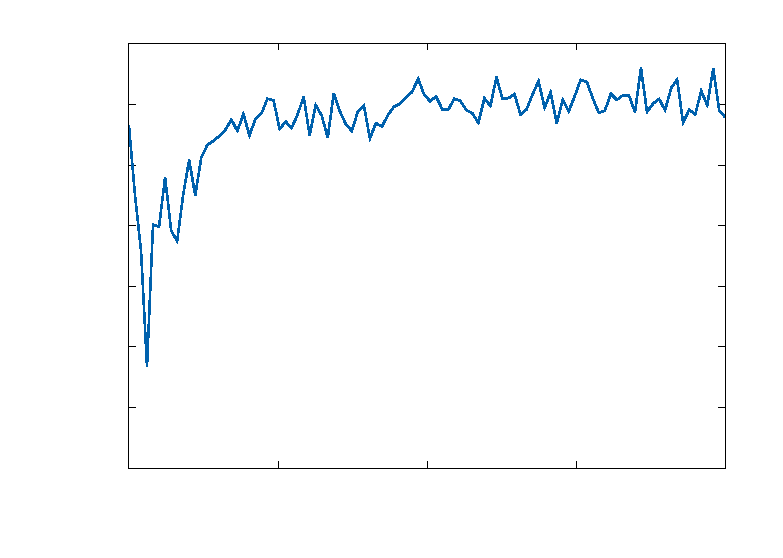
\includegraphics[width=\columnwidth]{figures/rel_fact_err/rel_fact_err.tex}}
\caption{Relative factorization error rate grow with the number of iterations of FMCB.}
\end{center}
\label{fig:factorization-effectiveness}
\vskip -0.2in
\end{figure}

As stated before, the intuition tells that factorization effectiveness will be reduced with each step. Fig.~\ref{fig:factorization-effectiveness} illustrates this effect on example of segment data set (see Sec.\ref{datasets} for details). Factorization gives us the best approximation of $R_t$ in class of rank 1 matrices, so we need to change the optimization goal. There are at least two different approaches to this task: introducing noise into data or biasing the solution by some prior.

\paragraph{Regularization (FMCB-EN)} % (fold)
\label{par:regularization}

% paragraph paragraph_name (end)
In this approach we are to define what kind of solutions are preferred above the others. The modeling matrix column structure gives us idea on this: each class should be either totally excluded or have positive/negative label. In our terms this means sparsity of $b_t$ vector. The most popular prior in this case is Laplacian which gives us $l_1$ regularization term in regression task. On the other hand if we let the $r$ vector grow, this regularization won't be effective because norms of these vectors are balanced. To limit the growth of $r$ we introduce normal prior and $l_2$ regularization on $r$ term. The final task takes the following form:
\begin{multline}
(b_{t+1},r_{t+1}) = \arg \min_{b,r} \|b r^T - R_t\|_F + \lambda_1 \|b\|_1 + \lambda_2 \|r\|_2
\label{eq:factorization_l1}
\end{multline}
We employ alternating least squares idea to solve (\ref{eq:factorization_l1}). Both steps of the algorithm are similar to each other, lets suppose that $r$ is fixed:
\begin{multline*}
	\hat{b} = \arg\min_{b}\|R_t-br^T\|_2^{2} + \lambda_1 \|b\|_1 + \lambda_2 \|r\|_2^2 \\
	= \arg\min_{b}\sum_{c,i}\left(R_{tci}-b_cr_i\right)^{2} + \lambda_1 \|b\|_1
	\label{eq:elastic-net-argmin}
\end{multline*}
Therefore, we have reduced the initial problem to the linear regression with either $l_1$ or $l_2$ (in case of $r$) regularization, that could be generalized to \emph{Elastic-Net}. Indeed, it can be rewritten to canonical form:
 \begin{equation*}
x^{*}=\arg\min\Vert y-Ax\Vert_{2}^{2}+\lambda_{1}\Vert x\Vert_{2}^{2}+\lambda_{2}\Vert x\Vert_{1},\label{eq:elastic-net-canon-argmin}
\end{equation*}
where $A \in \mathbb{R}^{|X|(K-1)\times |X|}$ and $y \in \mathbb{R}^{|X|(K-1)}$:
\[
A =
\begin{pmatrix}
	b_{1}     		& 				&		  \\
	\vdots			& \mathbb{O}  	&		  \\
	b_{K-1}			& 				&		  \\
					& \ddots		&		  \\
					&   			& b_{1}	  \\
					& \mathbb{O}	& \vdots  \\
					& 				& b_{K-1}
\end{pmatrix},
y=\begin{pmatrix}\begin{array}{l}
	\nabla R_{t1,1}		\\
	\vdots				\\
	\nabla R_{t1,K-1}	\\

	\vdots				\\
	
	R_{t|X|,1}		\\
	\vdots				\\
	R_{t|X|,K-1}
\end{array}\end{pmatrix}
\]
Detailed algorithm for \emph{Elastic-Net} problem could be found at \cite{Hastie_theelements} or \cite{elasticnet05}.

\paragraph{Columns sampling (FMCB-CS)}
On each iteration we "disable" random columns of the gradient's matrix by setting them to zero with probability $\frac{1}{K}$. It ensures that singular values will be "shake-up" and consequently it particularly protects us from the problem described above. However, this approach is very unstable and may cause method divergence.

\begin{figure}
\vskip 0.2in
\begin{center}
\centerline{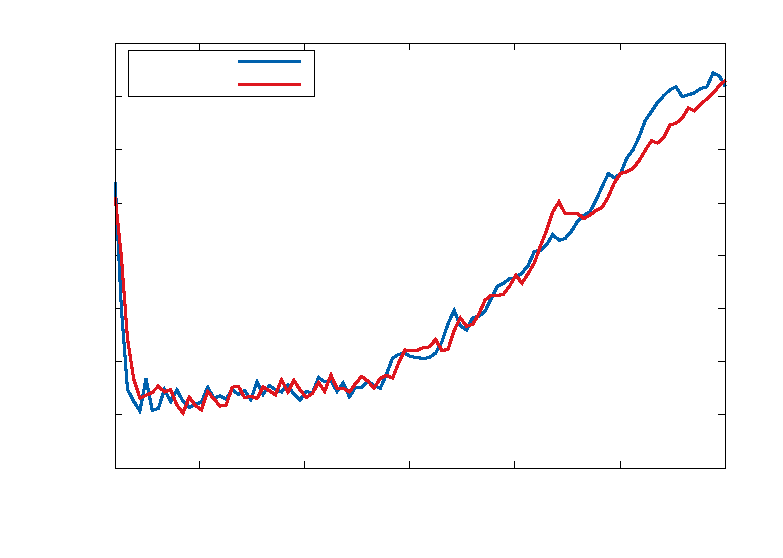
\includegraphics[width=\columnwidth]{figures/cn/cn.tex}}
\caption{Condition number of the gradient matrix during training FMCB and FMCB-EN models on \emph{pendigits} dataset.}
\end{center}
\label{fig:condition_number}
\vskip -0.2in
\end{figure}

\paragraph{Effect of the bias}
To evaluate effect of the bias introduction we track the condition number of the matrix $R_t$ which determines the quality of the factorization. The Fig.~\ref{fig:condition_number} shows the effect of our manipulations. Several first iterations are taken out from the graph because of the scaling problems (condition number is too big). As one can see, effect of bias introduction is fairy small and looking for more effective ways to deal with factorization quality degradation is one of the most promising directions of the future work. Interesting fact is that after certain number of iterations the condition number starts to grow. The norm of the gradient at that point starts to be so low, that successive iteration gradients are not aligned with each other. At that point original algorithm starts to be more precise. The problem is that this point could be not reached at some collections.

\begin{figure}
\vskip 0.2in
\begin{center}
\centerline{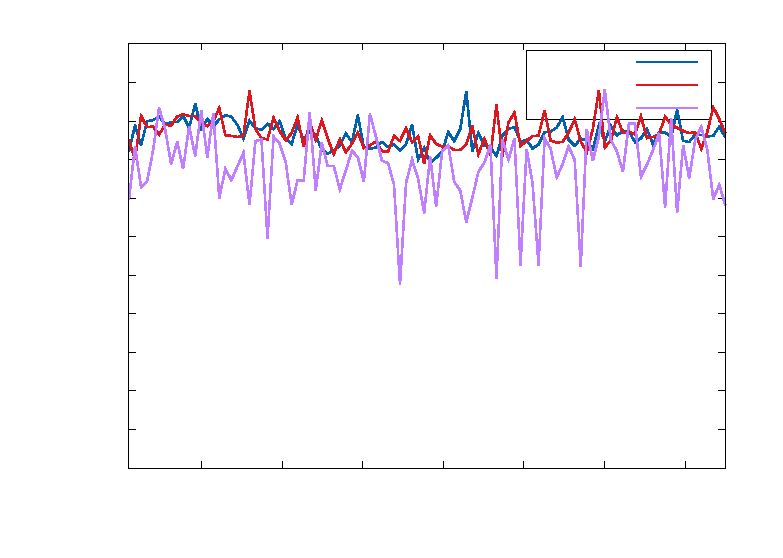
\includegraphics[width=\columnwidth]{figures/grad_norm/gradnorm.tex}}
\caption{Gradient norm by iterations count for all proposed modifications.}
\end{center}
\label{fig:gradient_norm}
\vskip -0.2in
\end{figure}

\paragraph{Convergence}
As stated in Sec.~\ref{sec:fmcb_idea} two step optimization of the $R_t$ does not allow us to say anything on convergence of the proposed method. The other problem is that factorization error rate is pretty high (see Fig.~\ref{fig:factorization-effectiveness}). Considering it in couple with the residual of the (\ref{eq:minimization_step}) the effective direction of the $b h_t(X)^T$ could be far from original $R_t$ and lead to $H$ quality reduction. On the other hand we have easy way to ensure that this reduction have not happen yet: if $\|R_{t+1}\|_F <\|R_{t}\|_F$ then the last step was successful. This statement could be used as a stop condition for the algorithm. In the Fig.~\ref{fig:gradient_norm} one can see the drop of the gradient norm with the iterations count for proposed modifications of the algorithm.


\section{Experiments} \label{experiments}
Let us remind that our goal is to maximize the ratio between weak models count and prediction quality. In each experiment we compare accuracy that could be reached with fixed count of weak models. We have chosen two competing methods that could use the same weak model optimization: one vs. rest and multinomial logistic regression. This approach gives us the opportunity to compare the influence of the learning procedure but not the quality of the base/weak models.

We have tested the \emph{Factorized MultiClass Boosting} algorithm with data from the UCI repository \cite{uciRepo}. Table \ref{datasets} shows characteristics of different datasets used. Our goal was to compare proposed method and its competitors in principally different setups and chosen datasets allow us to do that.

\begin{table}[t]
\caption{Statistics for the classification datasets.}
\label{datasets}
\vskip 0.15in
\begin{center}
\begin{small}
\begin{sc}
\begin{tabular}{lrrrr}
\hline
\abovespace\belowspace
Data set & Examples & Features & Classes \\
\hline
\abovespace
wine     		& 178 	& 17 	& 3     \\
letter    		& 20000 & 16 	& 26 	\\
MNIST     		& 60000 & 785 	& 10    \\
pendigits 		& 7494 	& 21 	& 10 	\\
segmentation    & 2300 	& 23 	& 7     \\
\hline
\end{tabular}
\end{sc}
\end{small}
\end{center}
\vskip -0.1in
\end{table}

\documentclass{standalone}

\begin{document}

% what's going on here: we have 5 tables with detailed results for 4 models: mll, gf, gfen, ovr. 

% Format:
% trees	mll_scores
%		gf_scores
%		gfen_scores
%		ovr_scores
%
% where scores have format: (mf_mean+mf_std [mf_low_ci, mf_high_ci]) / (MF_mean+MF_std [MF_low_ci, MF_high_ci])
% (mf - micro_f1, MF - macro_f1)

% ./letters/table
% models	mll	gf	gfen	ovr
% 3120	(0.914822+0.005035 [0.911918, 0.917485]) / (0.915615+0.005467 [0.911969, 0.918473])
% 		(0.946169+0.005010 [0.941041, 0.948078]) / (0.946278+0.004943 [0.941958, 0.948450])
% 		(0.946777+0.001795 [0.945645, 0.947726]) / (0.947035+0.001689 [0.945966, 0.947933])
% 		(0.921943+0.005899 [0.918363, 0.925238]) / (0.922707+0.005990 [0.919316, 0.926178])

% 6240 	(0.933456+0.003572 [0.931149, 0.935462]) / (0.933770+0.003819 [0.931251, 0.935766])
% 		(0.957867+0.004170 [0.955297, 0.960067]) / (0.957763+0.004111 [0.955000, 0.959936])
% 		(0.958166+0.003105 [0.956169, 0.959777]) / (0.958205+0.002980 [0.956347, 0.959789])
% 		(0.943438+0.004180 [0.940277, 0.945539]) / (0.943637+0.004080 [0.940802, 0.945865])

% 9100 	(0.940391+0.004779 [0.937782, 0.943342]) / (0.940551+0.004921 [0.937378, 0.943559])
% 		(0.960252+0.004313 [0.957661, 0.962672]) / (0.960131+0.004205 [0.957312, 0.962447])
% 		(0.962153+0.003978 [0.959672, 0.964203]) / (0.962191+0.003894 [0.959684, 0.964345])
% 		(0.949729+0.003861 [0.947195, 0.951839]) / (0.949843+0.003851 [0.947554, 0.951811])
%
%
% ./mnist/table
% models	mll	gf	gfen	ovr
% 1300	(0.952298+0.002039 [0.950951, 0.953415]) / (0.951944+0.002199 [0.950622, 0.953087])
% 		(0.963547+0.001552 [0.962680, 0.964472]) / (0.963269+0.001584 [0.962389, 0.964150])
% 		(0.963399+0.002231 [0.962294, 0.964944]) / (0.963132+0.002305 [0.962024, 0.964707])
% 		(0.956639+0.001884 [0.955551, 0.957643]) / (0.956340+0.001933 [0.955231, 0.957387])
%
% 2600	(0.962831+0.001699 [0.962050, 0.964088]) / (0.962553+0.001814 [0.961614, 0.963935])
% 		(0.969786+0.001350 [0.968934, 0.970576]) / (0.969594+0.001367 [0.968732, 0.970388])
% 		(0.970315+0.001913 [0.969208, 0.971365]) / (0.970097+0.001961 [0.969039, 0.971306])
% 		(0.966071+0.001519 [0.965120, 0.966883]) / (0.965867+0.001573 [0.964918, 0.966798])
%
% 4000	(0.967199+0.001689 [0.966281, 0.968246]) / (0.966944+0.001746 [0.965954, 0.967985])
% 		(0.972119+0.001390 [0.971332, 0.972956]) / (0.971953+0.001411 [0.971169, 0.972880])
% 		(0.973041+0.001845 [0.972067, 0.974220]) / (0.972860+0.001919 [0.971871, 0.974137])
% 		(0.970321+0.001420 [0.969258, 0.971026]) / (0.970148+0.001494 [0.969143, 0.970938])
%
%
% ./pendigits/table
% models	mll	gf	gfen	ovr
% 1300 	(0.987849+0.003195 [0.985768, 0.989564]) / (0.987961+0.003097 [0.986129, 0.989690])
% 		(0.990757+0.003586 [0.988916, 0.993002]) / (0.990934+0.003606 [0.989115, 0.993310])
% 		(0.991691+0.002887 [0.990033, 0.993393]) / (0.991835+0.002902 [0.990155, 0.993538])
% 		(0.990381+0.002695 [0.988877, 0.992011]) / (0.990605+0.002694 [0.988918, 0.992193])

% 2600 	(0.990120+0.002764 [0.988160, 0.991515]) / (0.990199+0.002694 [0.988454, 0.991553])
% 		(0.992091+0.003515 [0.990314, 0.994505]) / (0.992210+0.003566 [0.990215, 0.994266])
% 		(0.992899+0.003129 [0.991190, 0.994921]) / (0.992982+0.003196 [0.991118, 0.994934])
% 		(0.991193+0.002202 [0.989883, 0.992503]) / (0.991387+0.002196 [0.990171, 0.992635])

% 4000 	(0.990920+0.002580 [0.989103, 0.992266]) / (0.991033+0.002504 [0.989523, 0.992301])
% 		(0.992492+0.003497 [0.990842, 0.994948]) / (0.992633+0.003522 [0.990724, 0.995013])
% 		(0.993165+0.003205 [0.991293, 0.995172]) / (0.993283+0.003266 [0.991238, 0.995244])
% 		(0.991592+0.001804 [0.990603, 0.992715]) / (0.991750+0.001847 [0.990752, 0.992981])
%
%
% ./segment/table
% models	mll	gf	gfen	ovr
% 490 	(0.980592+0.010208 [0.974959, 0.986503]) / (0.980757+0.009923 [0.975127, 0.986661])
% 		(0.983644+0.008410 [0.979058, 0.988461]) / (0.984047+0.007319 [0.979819, 0.988265])
% 		(0.985342+0.007251 [0.981135, 0.989298]) / (0.986007+0.006244 [0.982566, 0.990045])
% 		(0.977452+0.008241 [0.973425, 0.983266]) / (0.977640+0.008533 [0.973782, 0.983643])

% 1050 	(0.981906+0.008462 [0.977106, 0.987422]) / (0.982009+0.008565 [0.977393, 0.987619])
% 		(0.984063+0.007776 [0.979216, 0.988166]) / (0.984386+0.006915 [0.980569, 0.988273])
% 		(0.985749+0.007579 [0.981013, 0.989848]) / (0.986255+0.006530 [0.982097, 0.989978])
% 		(0.979655+0.008432 [0.974750, 0.984958]) / (0.979733+0.008863 [0.974777, 0.985046])

% 1750 	(0.981823+0.009336 [0.976495, 0.987683]) / (0.981843+0.009565 [0.976761, 0.987241])
% 		(0.985325+0.007602 [0.980448, 0.989503]) / (0.985692+0.006752 [0.981548, 0.989411])
% 		(0.985749+0.007579 [0.980495, 0.989627]) / (0.986255+0.006530 [0.981428, 0.989473])
% 		(0.981379+0.007905 [0.976002, 0.985521]) / (0.981574+0.008253 [0.976158, 0.985744])
%
%
% ./wine/table
% models	mll	gf	gfen	ovr
% 30	(0.948882+0.046854 [0.923803, 0.975400]) / (0.947801+0.047724 [0.921972, 0.976582])
% 		(0.947671+0.040697 [0.925487, 0.970770]) / (0.925152+0.105859 [0.810031, 0.966517])
% 		(0.931409+0.050906 [0.900136, 0.959113]) / (0.909683+0.104691 [0.813619, 0.951616])
% 		(0.944808+0.084621 [0.881960, 0.984127]) / (0.951091+0.073016 [0.892577, 0.984604])

% 60	(0.969570+0.036525 [0.943902, 0.988235]) / (0.972358+0.034144 [0.946635, 0.987293])
% 		(0.967433+0.038717 [0.940616, 0.986425]) / (0.969948+0.035840 [0.945056, 0.987754])
% 		(0.954875+0.059847 [0.909626, 0.980912]) / (0.958142+0.054466 [0.914815, 0.984109])
% 		(0.950690+0.066832 [0.899690, 0.979365]) / (0.953682+0.059857 [0.910496, 0.981186])

% 90	(0.975126+0.036504 [0.946784, 0.992593]) / (0.976593+0.034738 [0.948554, 0.992172])
% 		(0.969243+0.046068 [0.937248, 0.991534]) / (0.970620+0.043485 [0.937444, 0.989167])
% 		(0.954875+0.059847 [0.905637, 0.982066]) / (0.958142+0.054466 [0.924120, 0.984178])
% 		(0.955452+0.068638 [0.898813, 0.988889]) / (0.958565+0.061596 [0.911335, 0.986070])



\begin{table*}%[t]
\label{exp-results}
\centering
\caption{Micro-averaged $F_{1}$ scores for the multinomial logistic regression (MLR), factorized multiclass boosting (FMCB), factorized multiclass boosting with elastic-net (FMCB-EN), factorized multiclass boosting with columns sampling (FMCB-CS), One-vs-Rest (OVR) models on benchmark datasets.}
\vskip 0.15in
\begin{small}
\begin{sc}
{\renewcommand{\arraystretch}{1.2}% for the vertical padding
\begin{tabular}{|l|c|c|c|c|c|c|}
\hline
\abovespace\belowspace
Dataset		& \# Models 	& MLR & FMCB & FMCB-EN 	& FMCB-CS & OVR  \\
\hline\hline
\multirow{3}{*}{wine}
	& 30    		& 0.949 $\pm$ 0.047 		 & 0.948 $\pm$ 0.041 & 0.931 $\pm$ 0.051 & \textbf{0.956 $\pm$ 0.002} & 0.945 $\pm$ 0.085\\
	& 60	  		& \textbf{0.970 $\pm$ 0.037} & 0.967 $\pm$ 0.039 & 0.955 $\pm$ 0.060 & 0.956 $\pm$ 0.002 & 0.951 $\pm$ 0.067\\
	& 90    		& \textbf{0.975 $\pm$ 0.037} & 0.969 $\pm$ 0.046 & 0.955 $\pm$ 0.060 & 0.963 $\pm$ 0.002 & 0.955 $\pm$ 0.069\\
\hline
\multirow{3}{*}{letters}
	& 3120			& 0.915 $\pm$ 0.005 & 0.946 $\pm$ 0.005 & \textbf{0.947 $\pm$ 0.002} & 0.947 $\pm$ 0.003 & 0.922 $\pm$ 0.006\\
	& 6240	 		& 0.933 $\pm$ 0.004 & 0.958 $\pm$ 0.004 & \textbf{0.958 $\pm$ 0.003} & 0.958 $\pm$ 0.003 & 0.943 $\pm$ 0.004\\
	& 9100 			& 0.940 $\pm$ 0.005 & 0.960 $\pm$ 0.004 & \textbf{0.962 $\pm$ 0.004} & 0.961 $\pm$ 0.004 & 0.950 $\pm$ 0.004\\
\hline
\multirow{3}{*}{mnist}
	& 1300			& 0.952 $\pm$ 0.002 & 0.964 $\pm$ 0.002 			& 0.963 $\pm$ 0.002 			& \textbf{0.964 $\pm$ 0.002} & 0.957 $\pm$ 0.002\\
	& 2600			& 0.963 $\pm$ 0.002 & 0.970 $\pm$ 0.001 	& 0.970 $\pm$ 0.002 			& \textbf{0.971 $\pm$ 0.002} & 0.966 $\pm$ 0.002\\
	& 4000			& 0.967 $\pm$ 0.002 & 0.972 $\pm$ 0.001 			& 0.973 $\pm$ 0.002 	& \textbf{0.973 $\pm$ 0.002} & 0.970 $\pm$ 0.001\\
\hline
\multirow{3}{*}{pendigits}
	& 1300			& 0.988 $\pm$ 0.003 & 0.991 $\pm$ 0.004 & \textbf{0.992 $\pm$ 0.003} & 0.991 $\pm$ 0.003 & 0.990 $\pm$ 0.003 \\
	& 2600			& 0.990 $\pm$ 0.003 & 0.992 $\pm$ 0.004 & \textbf{0.993 $\pm$ 0.003} & 0.992 $\pm$ 0.003 & 0.991 $\pm$ 0.002 \\
	& 4000			& 0.991 $\pm$ 0.003 & 0.992 $\pm$ 0.003 & \textbf{0.993 $\pm$ 0.003} & 0.992 $\pm$ 0.004 & 0.992 $\pm$ 0.002 \\
\hline
\multirow{3}{*}{segmentation}
	& 490			& 	0.981 $\pm$ 0.010 & 0.984 $\pm$ 0.008 & \textbf{0.985 $\pm$ 0.007} & 0.974 $\pm$ 0.003 & 0.977 $\pm$ 0.008 \\
	& 1050			& 	0.982 $\pm$ 0.008 & 0.984 $\pm$ 0.008 & \textbf{0.986 $\pm$ 0.008} & 0.975 $\pm$ 0.004 & 0.980 $\pm$ 0.008 \\
	& 1750			& 	0.982 $\pm$ 0.009 & 0.985 $\pm$ 0.008 & \textbf{0.987 $\pm$ 0.008} & 0.975 $\pm$ 0.004 & 0.981 $\pm$ 0.008 \\
\hline
\end{tabular}
\vskip -0.1in
} % {\renewcommand{\arraystretch}{1.2}% for the vertical padding
\end{sc}
\end{small}
\end{table*}
	





\end{document}
 
The results are presented in Table 2. Each cell contains mean and standard deviation of the accuracy evaluated with 10-folds cross-validation. We find that proposed algorithm FMCB almost always achieves the highest score compared to other models. Also we see that in the most of the cases we could sufficiently reduce the weak models count for FMCB variations methods and stay competitive with state-of-the-art methods in terms of prediction quality.

\section{Conclusions and future work}
In this paper we have presented new approach to multiclass classification problem. The proposed algorithms are able to be statistically significant better than multinomial logistic regression boosting and one vs. rest using the same weak learners. This advantage persists over collections we used for testing. The number of test collections does not allow us to say that the proposed method is always better in terms of prediction quality, but we have not found evidence of the opposite statement. The resulting decision function is computationally more lightweight than one for existing methods due to its' single ensemble nature. The computational difficulty of learning procedure is on par with one vs. rest and could be optimized even further, using more effective approximate factorization techniques. FMCB method is able to work with lot of classes and the only limitation is computational complexity of the matrix form of gradient factorization procedure.

Two major problems of the proposed approach were discovered:
\begin{itemize}
	\item the factorization error rate grows with the number of iterations;
	\item because of factorization error and non zero weak optimization residual the method is able to diverge.
\end{itemize}
To overcome the first difficulty we tested two methods of bias introduction in factorization task. The tested methods were able to soften, but not to eliminate the growth of the error rate. During this testing we have found that for certain collections the discovered problem is relevant only for limited number of iterations. The second problem could be practically solved by introduction of the stop condition. We have suggested such a condition and found that we were unable to reach it on test collections.

FMCB method tends to be both easy to use, it does not require thorough data preparation, and effective in terms of computational complexity to prediction quality ratio. We hope it could be used as a ``first attempt'' method for multiclass classification tasks.

As stated before we see the following three directions of further improvements:
\begin{itemize}
	\item factorization error elimination;
	\item reduction of the factorization computational cost;
	\item applying of the presented approach in multi-label setting.
\end{itemize}
The implementation of the algorithm could be found at github \cite{github}.
% We have described our vision on first problem solutions in the paper and now focus on the second. The matrix $R_t$ often have not even dimensions. In many cases $|X| >> K$ and one can interpret factorization process in probabilistic framework:
% $$
% \hat{b} = \arg \min_b \mathbb{E}_{r \in R_t}\sum_c\left(b_c \frac{\sum_c r_c}{\sum_c b_c} - r_c\right)^2
% $$
% This optimization could be done stochastically which is less computationally difficult. Besides the computation cost this allows us not to store $R_t$ matrix which is expansive in terms of memory consumption.
% main advantage of the \emph{GradFac} algorithm is the independence of the number of classes on the training stage: it's only required to train a single model instead of $K-1$ models. However, factorization stage depends on the number of classes. 
% Consider impact of factorization on quality of the final classification model. Obviously, matrix factorization increases total error because of replacement the whole matrix to outer product of two estimated vectors $u$ and $v$. Should we decrease the algorithm's quality on purpose? To answer this question one should remember the ability of the gradient boosting method to accumulate weak models in order to obtain the strong. Therefore, to compensate introduced error, we have to increase boosting iterations count and train some additional weak models (\emph{one} per iteration). 
% Suppose $L(H_{T}(x) \arrowvert X,Y) \le \varepsilon$ is true for the source algorithm after $T_{1}$ iterations and for the \emph{GradFac} algorithm after $T_{2}$ iterations. Note that $T_{1}<T_{2}$ because we need to compensate factorization error. Also note that the source algorithm requires to train $K-1$ weak models and the \emph{GradFac} algorithm requires to train $1$ model. It's hard to say definitely which model includes less weak models count: 
% \[
% \begin{array}{rccc}
% 	\text{Iterations count:}	& T_{1} 				& <		& T_{2} \\
% 	\text{Weak models count:}	& T_{1}\times(K-1) 		& ??	& T_{2}
% \end{array}
% \]
% We will come back to this issue in the experiments section.



% We have introduced in this paper a new multiclassification algorithm GradFac that is based on the idea of gradient's matrix factorization. Experiments demonstrated that our algorithm allows to build up to 3 times easier model than state-of-the-art models like OVR or MLR without quality degradation. Of course, more experiments are needed to better understand applicability limits of this method, especially for tasks with large class count.

% There are several avenues for future research. One of the most simple ideas - variation of considering eigen vectors count (instead of 1). GradFac is also appealing for multi-label tasks because there are several target functions for such tasks \cite{Tsoumakas07multi-labelclassification} that allow to represent their gradients as matrix and consequently allow to apply factorization techniques.

% \clearpage
% Acknowledgements should only appear in the accepted version. 
% \section*{Acknowledgments} 


% In the unusual situation where you want a paper to appear in the
% references without citing it in the main text, use \nocite
%\nocite{langley00}

\nocite{Hastie_theelements}
\nocite{GLM}
\nocite{Friedman98additivelogistic}
\nocite{Friedman00greedyfunction}
\nocite{Zhao_sparseoutput}
\nocite{Allwein00reducingmulticlass}
\nocite{Crammer00onthe}
\nocite{Rifkin04indefense}
\nocite{Lee01algorithmsfor}
\nocite{Koren09matrixfactorization}
\nocite{Hu08collaborativefiltering}
\nocite{Gulin_winningthe}
\nocite{Eckart1936}
\nocite{elasticnet05}
\nocite{Efron1992bootstrap}
%\nocite{multilabel12}
\nocite{uciRepo}

\bibliography{example_paper}
\bibliographystyle{icml2017}

\end{document} 